\chapter*{Acknowledgments}\label{C:ack} 
Thank you Danny B for being great :- ) 

Thank you ECS Techs for putting up with my questions 

And thank you to my wonderful girlfriend for not kicking me out when I was working on this stupid fucking project really late 


% \chapter{Project Proposal}\label{A:proposal}

% % Include the entire project proposal document
% 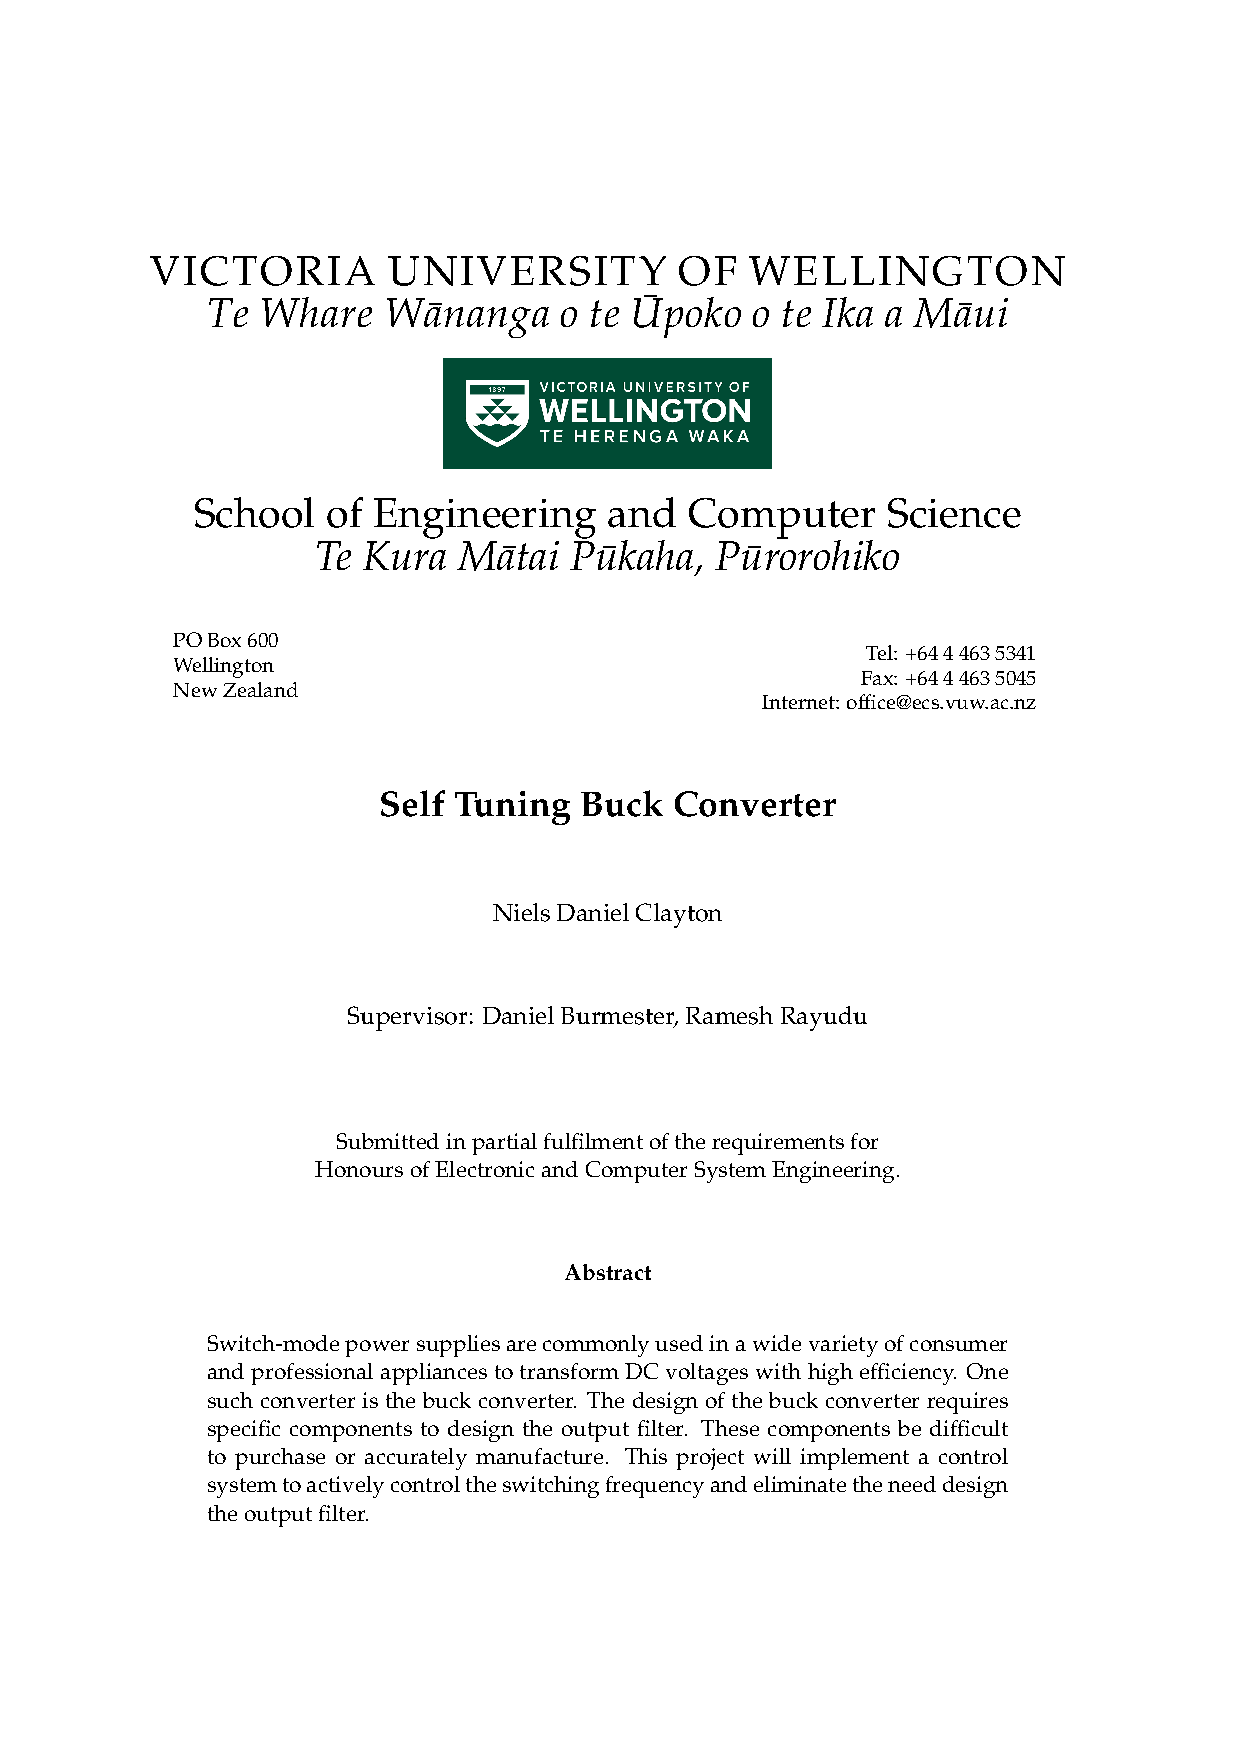
\includepdf[pages=-]{../Project\ Proposal/proj_proposal.pdf}

% Please add the following required packages to your document preamble:
% \usepackage[table,xcdraw]{xcolor}
% If you use beamer only pass "xcolor=table" option, i.e. \documentclass[xcolor=table]{beamer}
\begin{table}[]
    \centering
    \begin{tabular}{|l|l|
    >{\columncolor[HTML]{DCFCDC}}l |l|
    >{\columncolor[HTML]{FCDADA}}l |}
    \hline
    \multicolumn{5}{|c|}{\cellcolor[HTML]{FFE4C3}\textbf{\begin{tabular}[c]{@{}c@{}}150mV  Peak to Peak Input Signal\\ Initial and Final Design Peak Detector Output Error Across Frequencies\end{tabular}}} \\ \hline
    \textbf{Frequency (kHz)}         & \textbf{Final Design Error (mV)}        & \textbf{Final Design \% Error}        & \textbf{Initial Design Error (mV)}        & \textbf{Initial Design \% Error}        \\ \hline
    1                                & -3.90                                   & -5.2                                  & 3.40                                      & 4.533333333                             \\ \hline
    5                                & -3.80                                   & -5.066666667                          & 5.80                                      & 7.733333333                             \\ \hline
    10                               & -3.70                                   & -4.933333333                          & 12.80                                     & 17.06666667                             \\ \hline
    15                               & -2.90                                   & -3.866666667                          & 18.50                                     & 24.66666667                             \\ \hline
    20                               & -2.20                                   & -2.933333333                          & 23.30                                     & 31.06666667                             \\ \hline
    25                               & -1.60                                   & -2.133333333                          & 28.30                                     & 37.73333333                             \\ \hline
    30                               & -0.90                                   & -1.2                                  & 32.60                                     & 43.46666667                             \\ \hline
    35                               & -0.30                                   & -0.4                                  & 36.50                                     & 48.66666667                             \\ \hline
    40                               & 0.20                                    & 0.266666667                           & 40.20                                     & 53.6                                    \\ \hline
    45                               & 0.80                                    & 1.066666667                           & 43.70                                     & 58.26666667                             \\ \hline
    50                               & 1.30                                    & 1.733333333                           & 47.00                                     & 62.66666667                             \\ \hline
    55                               & 2.00                                    & 2.666666667                           & 50.10                                     & 66.8                                    \\ \hline
    60                               & 2.60                                    & 3.466666667                           & 53.00                                     & 70.66666667                             \\ \hline
    65                               & 3.10                                    & 4.133333333                           & 56.10                                     & 74.8                                    \\ \hline
    70                               & 3.50                                    & 4.666666667                           & 59.50                                     & 79.33333333                             \\ \hline
    75                               & 4.00                                    & 5.333333333                           & 62.70                                     & 83.6                                    \\ \hline
    80                               & 4.60                                    & 6.133333333                           & 65.20                                     & 86.93333333                             \\ \hline
    85                               & 5.00                                    & 6.666666667                           & 67.80                                     & 90.4                                    \\ \hline
    90                               & 5.60                                    & 7.466666667                           & 68.10                                     & 90.8                                    \\ \hline
    95                               & 6.10                                    & 8.133333333                           & 68.10                                     & 90.8                                    \\ \hline
    100                              & 6.70                                    & 8.933333333                           & 68.10                                     & 90.8                                    \\ \hline
    \end{tabular}
    \caption{Table of output errors at varying frequencies for both the initial and final peak detection design.}
    \label{T:150mV_peak_error}
    \end{table} 



\chapter{System Specification Derivation Equations} \label{A:specs}

The system specification derivation equations have been input into the graphing platform \url{Desmos.com}. This has allowed me to visually inspect these equations and form conclusions. The full working and step by step derivation is also available on \url{Desmos.com} using the following links.\\

Duty cycle equation derivation:\\
\url{https://www.desmos.com/calculator/8c7wmbyzw4}\\

Inductor sizing equation derivation:\\ 
\url{https://www.desmos.com/calculator/v7ntrescw5}\\

PWM frequency equation derivation:\\ 
\url{https://www.desmos.com/calculator/ekjhcrt9zg}\\

\chapter{Analogue PWM Generation} \label{A:analogue_PWM}


\begin{figure}[H]
    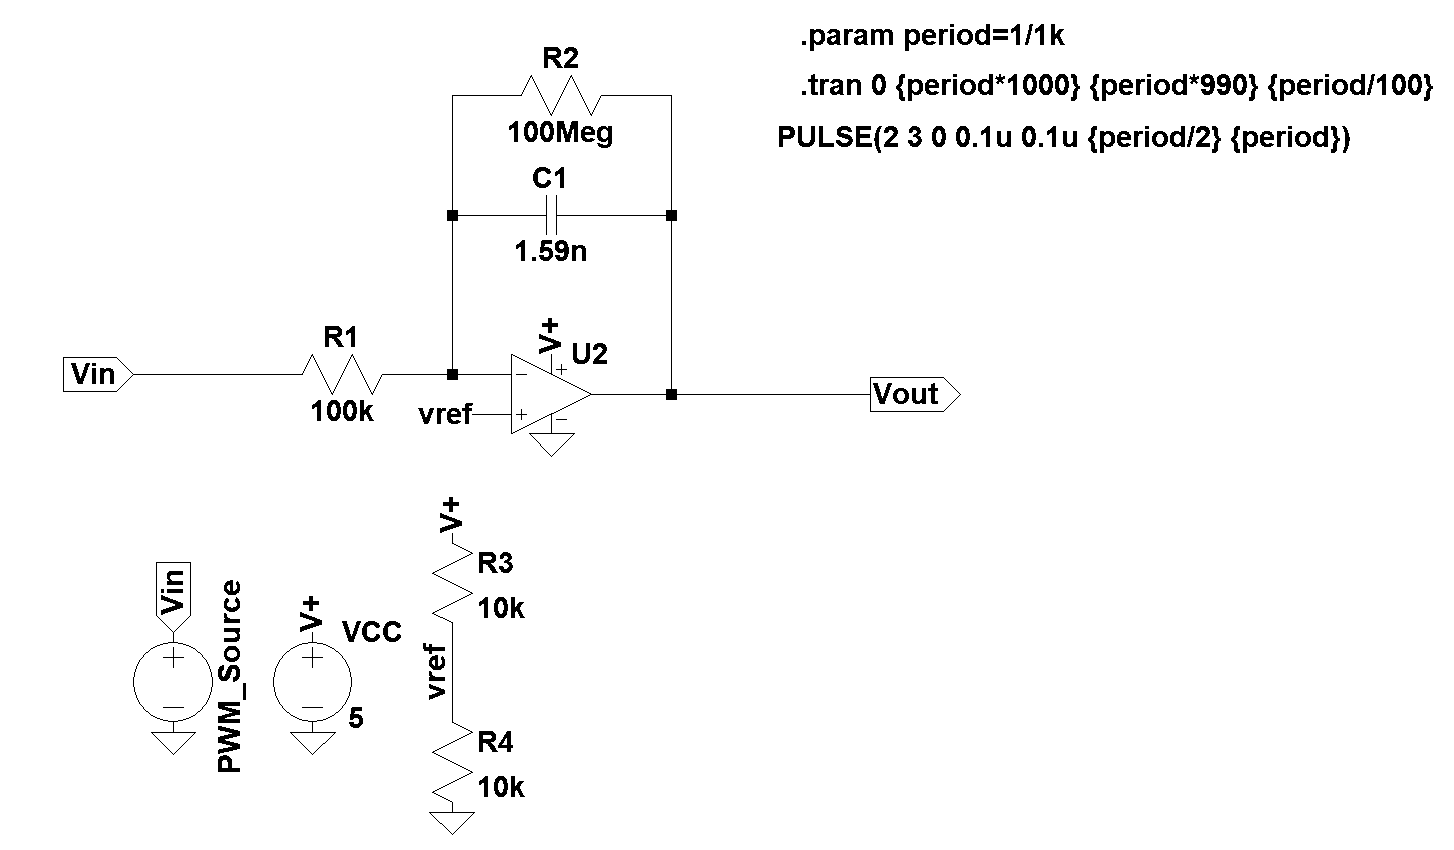
\includegraphics[width = 0.95\textwidth]{pwm/analog/analogue_PWM_ltspice_circuit.png}
    \caption{Analogue PWM LTSpice circuit}
\end{figure}

\begin{figure}[H]
    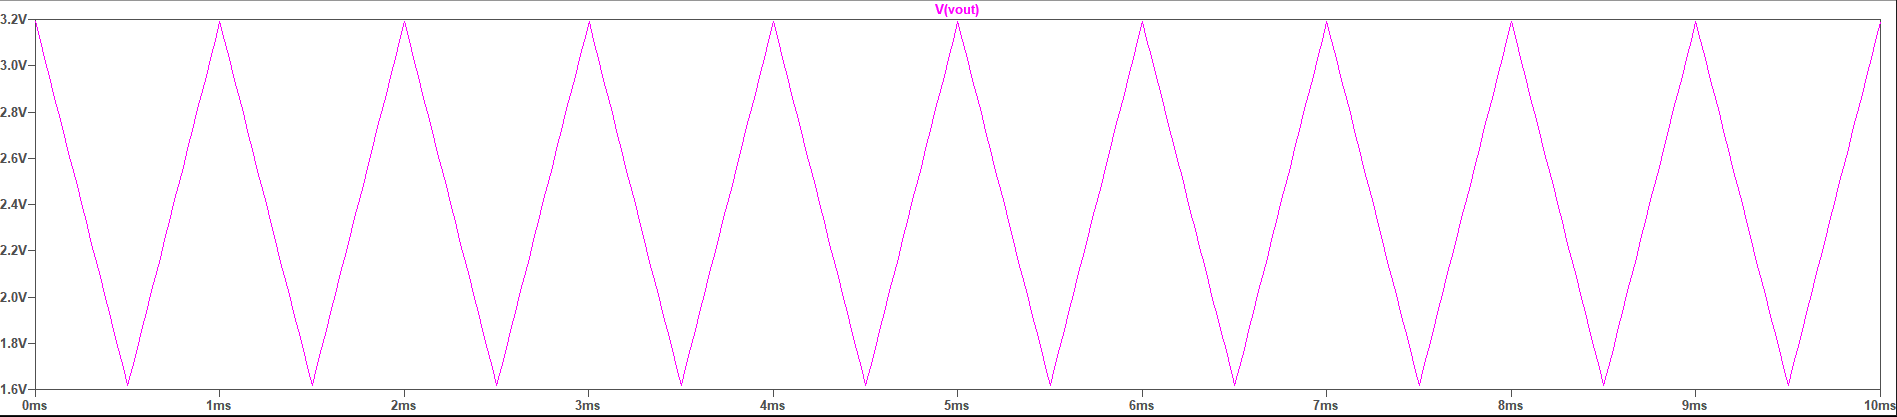
\includegraphics[width = 0.95\textwidth]{pwm/analog/analogue_PWM_ltspice_1k.png}
    \caption{Analogue PWM LTSpice simulation 1$kHz$}
\end{figure}

\begin{figure}[H]
    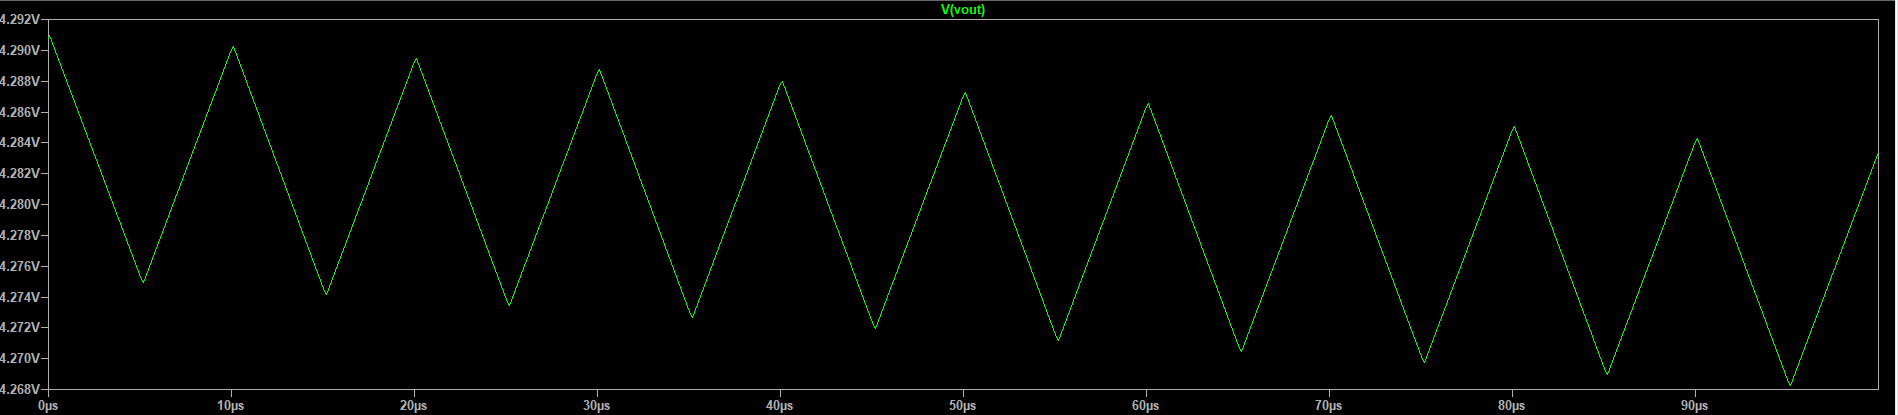
\includegraphics[width = 0.95\textwidth]{pwm/analog/analogue_PWM_ltspice_100k.png}
    \caption{Analogue PWM LTSpice simulation 100$kHz$}
\end{figure}


\chapter{Digital PWM Generation} \label{A:digital_PWM}

\section{Digital PWM Generation Figures}

\begin{figure}[H]
    \centering
    \begin{subfigure}{0.45\textwidth}
        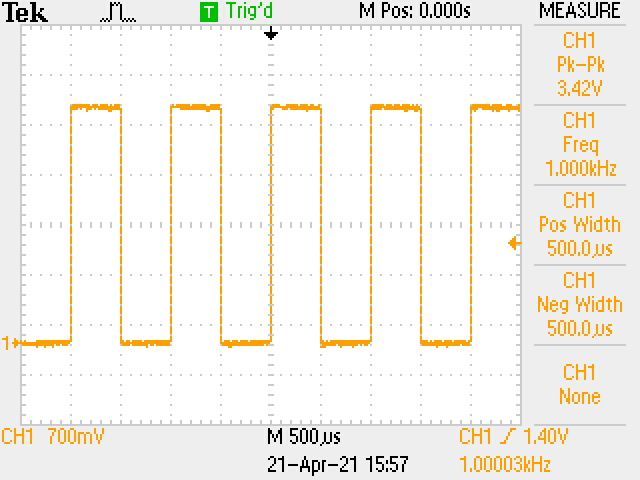
\includegraphics[width=\columnwidth]{pwm/duty/1kHz_50Duty.JPG}
        \subcaption{Digital PWM Generation at $1kHz$ and a 50\% duty cycle}

    \end{subfigure}
    \begin{subfigure}{0.45\textwidth}
        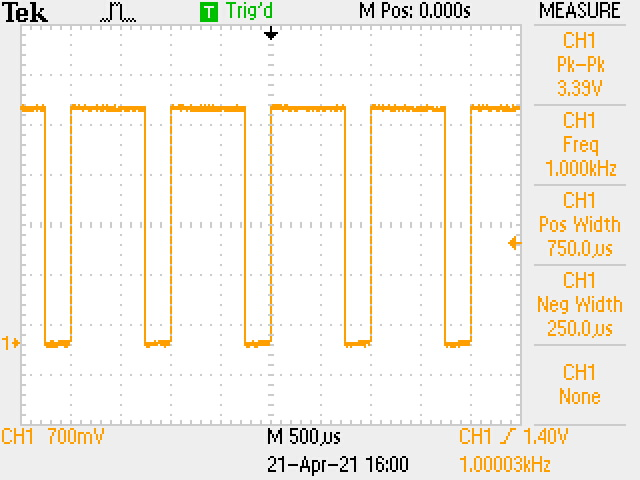
\includegraphics[width=\columnwidth]{pwm/duty/1kHz_75Duty.JPG}
        \subcaption{Digital PWM Generation at $1kHz$ and a 75\% duty cycle}

    \end{subfigure}
    \caption{Digital PWM Generation at $1kHz$}

\end{figure}

\begin{figure}[H]
    \centering
    \begin{subfigure}{0.45\textwidth}
        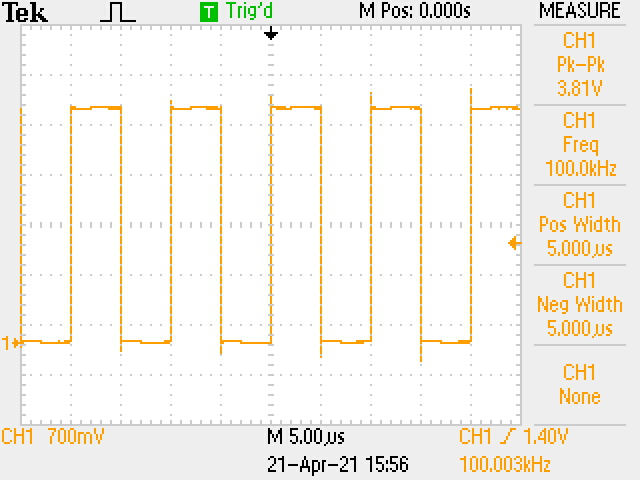
\includegraphics[width=\columnwidth]{pwm/duty/100kHz_50Duty.JPG}
        \subcaption{Digital PWM Generation at $100kHz$ and a 50\% duty cycle}

    \end{subfigure}
    \begin{subfigure}{0.45\textwidth}
        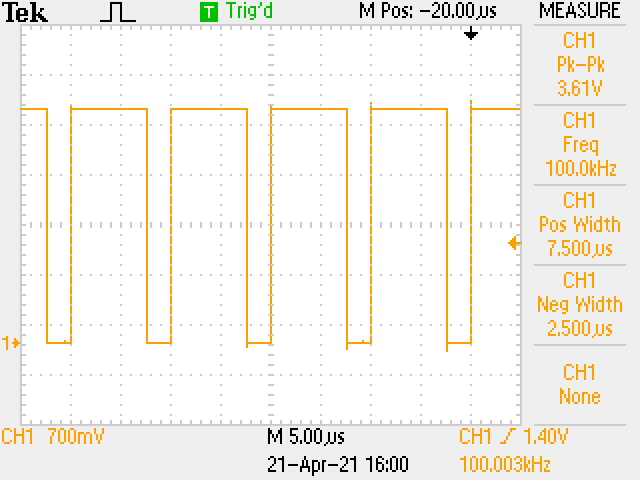
\includegraphics[width=\columnwidth]{pwm/duty/100kHz_75Duty.JPG}
        \subcaption{Digital PWM Generation at $100kHz$ and a 75\% duty cycle}

    \end{subfigure}
    \caption{Digital PWM Generation at $100kHz$}

\end{figure}

\newpage
\section{Digital PWM Generation Code}

\lstinputlisting{code/main.c}